\subsection{Valg af ledeskrue} \label{Valg af led screw og motor}
Det er i afsnit \ref{løsningsanal: Lineær bevægelse} valgt, at benytte en ledeskrue til de lineære bevægelser. Det er nødvendigt, at finde dimensioner på ledeskruen, samt dens gevindhældning, for at beregne variation på prikplacering og tidsforbruget, da disse afhænger af hældningen på gevindet. 
Gevindhældningen er den lineære afstand gevindet har bevæget sig ved en omgang, og er illustreret i figur \ref{fig: skrue forklaringer}. En højere gevindhældning vil resultere i længere lineær bevægelse per omgang. Det medfører også en lavere præcision, da en motor er begrænset i, hvor lille en vinkel den kan rotere sig.


\begin{figure}[H]
    \centering
    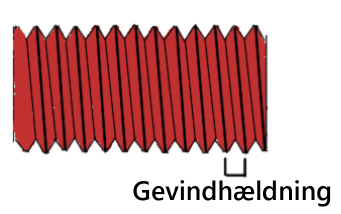
\includegraphics[width=0.4\linewidth]{Sections/6 Detaljeløsning/Media/skruer.png}
    \caption{Illustration gevindhældning}
    \label{fig: skrue forklaringer}
\end{figure} \plainbreak{-0.5}

Nøjagtigheden er også afhængig af motoren, både i forhold til eventuelle unøjagtigheder i motorens konstruktion, samt den mindste rotation den kan udføre. Da løsningen kommer til at skulle foretage mange små og præcise bevægelser kan der allerede nu konkluderes at en step-motor er bedst egnet til formålet. step-motorer rotere i steps i stedet for kontinuert, som en servomotor, dette betyder det er muligt at nøjagtigt kontrollere hvor meget motoren skal rotere. En fuld rotation er delt op i et antal steps, dette kaldes \textit{step antal}. Nogen fabrikanter vælger i stedet at oplyse hvor mange grader et step dækker, dette kaldes \textit{stepvinkel}

Grundet de geometriske begrænsning vælges det at motoren skal være af typen NEMA 14. Dette er en monterings standard fra National Electrical Manufacturers Association (NEMA). Denne størrelse motor har typisk en step antal på 200, og det er dette ledeskrue dimensioneres ud fra.

I HoQ blev der konkluderet at nøjagtighed er vigtigere end hastighed.  For at tage hensyn til begge kravs vigtighed, vælges der en ledeskrue med en gevindhældning på \SI{2}{mm}. Dette giver en maksimal afvigelse på \SI{0,01}{mm}, som opfylder præstationskrav 3 med en sikkerhedsfaktor på 10. Det vælges derudover, at skruen skal have en diameter på \SI{10}{mm}, da det vil give en større modstand imod udbøjning. \parencite{Igus2025DrylinSteel}




%Når gevindstigningen nævnes, menes der afstanden imellem hvert indhak i gevindet. Dette er det samme som gevindhældningen i tilfældet af, at skruen er en enkeltstartsskrue. Dette betyder at der skrues langs én linje i skruen, hvorimod dobbeltstart har to parallelle linjer på skruen der skrues langs, som det ses på figur \ref{fig: skrue forklaringer}. \parencite{Sild2022LeadFractory}